% STRIPE real-time pipeline — vector figure.
% Standalone: `pdflatex system_pipeline.tex`. Or copy the tikzpicture into the
% paper (needs \usetikzlibrary{positioning,fit,backgrounds,arrows.meta}).
\documentclass[border=6pt]{standalone}
\usepackage{tikz}
\usepackage{amsmath}
\usetikzlibrary{positioning,fit,backgrounds,arrows.meta}
\begin{document}
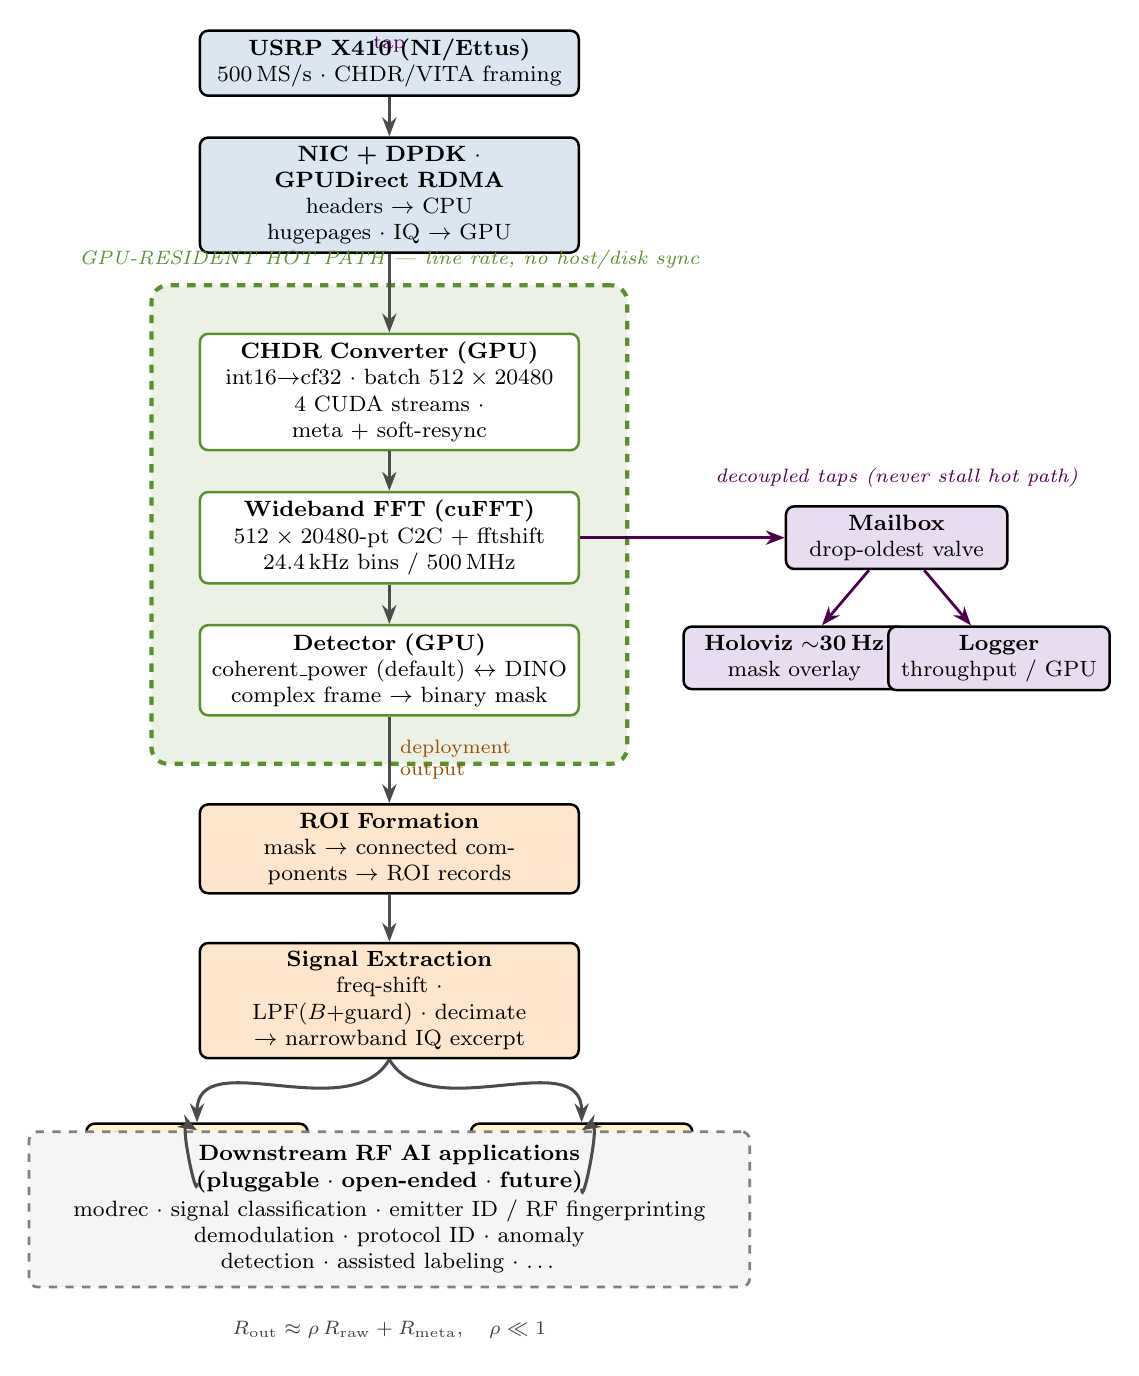
\begin{tikzpicture}[
  font=\footnotesize,
  >={Stealth[length=2.4mm]},
  box/.style={draw=#1, line width=0.9pt, rounded corners=3pt, align=center,
              text width=46mm, inner sep=3pt, fill=white},
  small/.style={draw=#1, line width=0.9pt, rounded corners=3pt, align=center,
              text width=26mm, inner sep=3pt, fill=white},
  flow/.style={->, line width=1.1pt, gray!60!black},
  tap/.style={->, line width=1.0pt, violet!60!black},
]
\definecolor{rfblue}{HTML}{DBE6F0}
\definecolor{gpugreen}{HTML}{5A8F2A}
\definecolor{roior}{HTML}{FDE6CC}
\definecolor{strym}{HTML}{FFF3CC}
\definecolor{dispp}{HTML}{E8DDF0}

% ---- main column ----
\node[box=black, fill=rfblue] (usrp) {\textbf{USRP X410 (NI/Ettus)}\\500\,MS/s $\cdot$ CHDR/VITA framing};
\node[box=black, fill=rfblue, below=5mm of usrp] (nic) {\textbf{NIC + DPDK $\cdot$ GPUDirect RDMA}\\headers $\to$ CPU hugepages $\cdot$ IQ $\to$ GPU};
\node[box=gpugreen, below=10mm of nic] (chdr) {\textbf{CHDR Converter (GPU)}\\int16$\to$cf32 $\cdot$ batch $512\times20480$\\4 CUDA streams $\cdot$ meta + soft-resync};
\node[box=gpugreen, below=5mm of chdr] (fft) {\textbf{Wideband FFT (cuFFT)}\\$512\times20480$-pt C2C + fftshift\\24.4\,kHz bins / 500\,MHz};
\node[box=gpugreen, below=5mm of fft] (det) {\textbf{Detector (GPU)}\\coherent\_power (default) $\leftrightarrow$ DINO\\complex frame $\to$ binary mask};
\node[box=black, fill=roior, below=11mm of det] (roi) {\textbf{ROI Formation}\\mask $\to$ connected components $\to$ ROI records};
\node[box=black, fill=roior, below=6mm of roi] (ext) {\textbf{Signal Extraction}\\freq-shift $\cdot$ LPF($B$+guard) $\cdot$ decimate\\$\to$ narrowband IQ excerpt};

\node[small=black, fill=strym, below left=8mm and -14mm of ext] (meta) {\textbf{ROI metadata}\\stream};
\node[small=black, fill=strym, below right=8mm and -14mm of ext] (iq) {\textbf{Selected IQ}\\snippets ($\rho\ll1$)};

\node[draw=gray, line width=1pt, dashed, rounded corners=3pt, align=center,
      text width=88mm, inner sep=5pt, fill=gray!8, below=9mm of ext] (down)
  {\textbf{Downstream RF AI applications\ \ (pluggable $\cdot$ open-ended $\cdot$ future)}\\[1pt]
   modrec $\cdot$ signal classification $\cdot$ emitter ID / RF fingerprinting\\
   demodulation $\cdot$ protocol ID $\cdot$ anomaly detection $\cdot$ assisted labeling $\cdot$ \dots};

% ---- decoupled display/log branch ----
\node[small=black, fill=dispp, right=26mm of fft] (mbox) {\textbf{Mailbox}\\drop-oldest valve};
\node[small=black, fill=dispp, below=7mm of mbox, xshift=-13mm] (holo) {\textbf{Holoviz $\sim$30\,Hz}\\mask overlay};
\node[small=black, fill=dispp, below=7mm of mbox, xshift=13mm] (log) {\textbf{Logger}\\throughput / GPU};

% ---- hot-path background ----
\begin{scope}[on background layer]
  \node[draw=gpugreen, line width=1.5pt, dashed, rounded corners=6pt,
        fill=gpugreen!12, fit=(chdr)(fft)(det), inner sep=6mm] (hot) {};
\end{scope}
\node[gpugreen, font=\scriptsize\itshape, above=0.5mm of hot.north]
  {GPU-RESIDENT HOT PATH --- line rate, no host/disk sync};

% ---- arrows ----
\draw[flow] (usrp) -- (nic);
\draw[flow] (nic) -- (chdr);
\draw[flow] (chdr) -- (fft);
\draw[flow] (fft) -- (det);
\draw[flow] (det) -- (roi) node[midway,right,font=\scriptsize,orange!60!black,align=left]{deployment\\output};
\draw[flow] (roi) -- (ext);
\draw[flow] (ext.south) to[out=-120,in=90] (meta.north);
\draw[flow] (ext.south) to[out=-60,in=90] (iq.north);
\draw[flow] (meta.south) to[out=-90,in=150] (down.north-|meta);
\draw[flow] (iq.south) to[out=-90,in=30] (down.north-|iq);
\draw[tap] (fft.east) to[out=0,in=180] (mbox.west) node[midway,above,font=\scriptsize,violet!60!black]{tap};
\draw[tap] (mbox) -- (holo);
\draw[tap] (mbox) -- (log);

\node[font=\scriptsize\itshape, violet!60!black, above=1mm of mbox] {decoupled taps (never stall hot path)};
\node[font=\scriptsize, gray!50!black, below=3mm of down] {$R_{\mathrm{out}}\approx\rho\,R_{\mathrm{raw}}+R_{\mathrm{meta}},\quad \rho\ll1$};
\end{tikzpicture}
\end{document}
